% !TEX root = ./problem.en.tex
\gdef\thisproblemauthor{}
\gdef\thisproblemdeveloper{}
\gdef\thisproblemorigin{}
\begin{problem}{磨樹 Woody}
{standard input}{standard output}
{0.5 seconds}{512 MB}{}

Woody 是一位有著美學堅持的伐木工 \newline
他擁有一座森林,裡面的樹木都擁有方形樹幹 ( 如此完美!) \newline
他每天都會進行一次將樹幹磨得更細的工程 \newline
對於每棵樹選取接近根部的一小段樹幹,依圖中方式磨細 \newline
\newline
更精確地說,每次取橫切面 ( 正方形 ) 的中點連線 \newline
形成成較小的,旋轉 45 度的方形 \newline
再將這個小方形以外的部分磨掉 \newline
\newline
已之樹幹在截面積 $ \leq A $ 時會倒掉 \newline
給定一棵樹在第 0 天時的寬度 $ L $ \newline
Woody 從第 1 天開始磨樹 \newline
求這顆樹在第幾天會於磨樹途中或恰結束時倒掉 \newline

\centerline{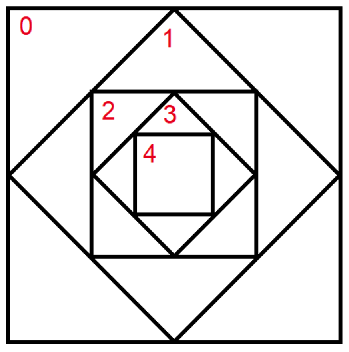
\includegraphics[scale=0.6]{./pics/A.png}}


\InputFile

輸入 2 個正整數 $ A $, $ L $ \newline
用空白分隔 \newline

\begin{iofmt}
\begin{itemize}
	\item $x_1\leq x_2$
	\item $y_1\leq y_2$
	\item $|x,y,x_1,x_2,y_1,y_2|\leq 10000$
\end{itemize}
\end{iofmt}

\OutputFile

請輸出夢想世界的面積,輸出到小數點後第$1$位。

\Examples

\begin{example}
\exmpfile{./sample/PA-in.txt}{./sample/PA-out.txt}%
\end{example}

\end{problem}
